\documentclass[10pt]{article}
\usepackage[polish]{babel}
\usepackage[utf8]{inputenc}
\usepackage[T1]{fontenc}
\usepackage{amsmath}
\usepackage{amsfonts}
\usepackage{amssymb}
\usepackage[version=4]{mhchem}
\usepackage{stmaryrd}
\usepackage{graphicx}
\usepackage[export]{adjustbox}
\graphicspath{ {./images/} }

\title{LIGA MATEMATYCZNA \\
 im. Zdzisława Matuskiego \\
 PAŹDZIERNIK 2022 \\
 SZKOŁA PONADPODSTAWOWA }

\author{}
\date{}


\begin{document}
\maketitle
\section*{ZADANIE 1.}
Czy istnieją liczby całkowite \(x, y, z\) takie, że \((3 x-5 y)(7 y-3 z)(3 z-x)=20222023\) ?

\section*{ZADANIE 2.}
Pola szachownicy \(9 \times 9\) pokolorowano w tradycyjny sposób, ale jej narożne pola są białe. Ruch polega na wybraniu dwóch sąsiednich pól i przemalowaniu ich na przeciwny kolor (to znaczy: jeżeli wybrane pole jest białe, to zmieniamy jego kolor na czarny, a gdy pole jest czarne, to zmieniamy jego kolor na biały). Czy można dobierać ruchy tak, aby w pewnym momencie wszystkie pola były czarne?

\section*{ZADANIE 3.}
Wierzchołki \(B, C\) trójkąta \(A B C\) połączono odcinkami z przeciwległymi bokami otrzymując małe trójkąty o polach 3, 3 i 1 (jak na rysunku). Oblicz pole trójkąta \(A B C\).\\
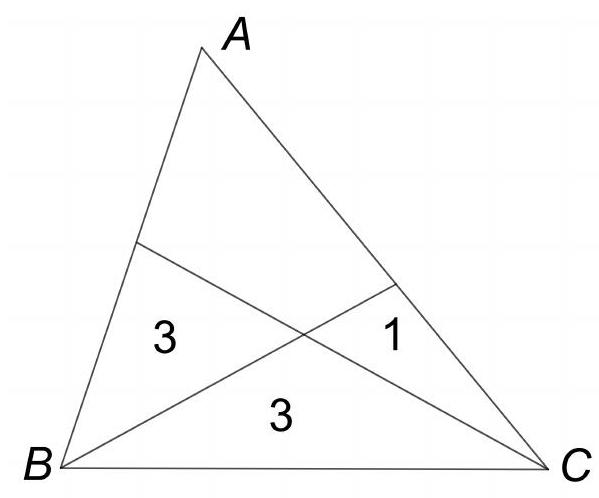
\includegraphics[max width=\textwidth, center]{2024_11_21_d499c641a0cc5271d18dg-1}

\section*{ZADANIE 4.}
Przedstaw liczbę 2023 jako różnicę kwadratów dwóch liczb naturalnych.

\section*{ZADANIE 5.}
W zbiorze liczb rzeczywistych rozwiąż układ równań

\[
\left\{\begin{array}{l}
x_{1}\left(x_{1}+x_{2}+x_{3}+x_{4}\right)=1 \\
\left(x_{1}+x_{2}\right)\left(x_{2}+x_{3}+x_{4}\right)=1 \\
\left(x_{1}+x_{2}+x_{3}\right)\left(x_{3}+x_{4}\right)=1 \\
\left(x_{1}+x_{2}+x_{3}+x_{4}\right) x_{4}=1
\end{array}\right.
\]


\end{document}